\documentclass[10pt,a4paper, margin=1in]{article}
\usepackage{fullpage}
\usepackage{amsfonts, amsmath, pifont}
\usepackage{amsthm}
\usepackage{graphicx}
\usepackage{float}

\usepackage{tkz-euclide}
\usepackage{tikz}
\usepackage{pgfplots}
\pgfplotsset{compat=1.13}
\begin{filecontents}{q5odd.dat}
 n   xn 
 1  -0.5
 -1   0.5
 2   1  
 -2 -1
 4 -2
 -4 2
 7 1.5
 -7 -1.5
\end{filecontents}
\begin{filecontents}{q5even.dat}
 n   xn 
 1  -0.5
 -1   -0.5
 2   1  
 -2 1
 4 -2
 -4 -2
 7 1.5
 -7 1.5
\end{filecontents}

\usepackage{geometry}
 \geometry{
 a4paper,
 total={210mm,297mm},
 left=10mm,
 right=10mm,
 top=10mm,
 bottom=10mm,
 }
 % Write both of your names here. Fill exxxxxxx with your ceng mail address.
 \author{
  Uzun, Yunus Emre\\
  \texttt{e2172104@ceng.metu.edu.tr}
  \and
  Vefa, Ahmet Dara\\
  \texttt{e2237899@ceng.metu.edu.tr}
}
\title{CENG 384 - Signals and Systems for Computer Engineers \\
Spring 2018-2019 \\
Written Assignment 1}

\begin{filecontents}{q1.dat}
 n   xn 
 -1  1
\end{filecontents}

\begin{filecontents}{q3a.dat}
 n   xn 
 -7  3
 -6  0
 -5  0
 -4 -4
 -3  0
 -2  2
 -1 -1
  0 -1
  1  0
  2  0
  3  3
\end{filecontents}

        
\begin{document}
\maketitle



\noindent\rule{19cm}{1.2pt}

\begin{enumerate}

\item 
    \begin{enumerate}
    % Write your solutions in the following items.
    \item 
        \begin{align*}
        &1& z = & x+ yj &\\
        &2& \Bar{z} = & x - yj & \\
        &3& 3z + 4 = & 2j - \Bar{z} & \\
        &4& 3x + 3yj +4 = & 2j - x + yj & \\
        &5& 4x + 4 = & 0 & (eqn. 1) \\
        &6& 2y = & 2 & (eqn. 2) \\
        &7& eqn1 \implies & x = -1 & \\
        &8& eqn2 \implies & y = 1 & \\
        &9& z = & -1+j &\\
        \end{align*}
        (i)  $|z|^2 = (-2(j^2)) = 2$ \\
        (ii) 
        \begin{figure}[h!]
            \centering
            \begin{tikzpicture}[scale=1.0]
               \begin{axis}[
              axis lines=middle,
              xlabel={$Re$},
              ylabel={$\boldsymbol{Im}$},
              xtick={-2, -1, ..., 2},
              ytick={-2, -1, ..., 2},
              ymin=-2, ymax=2,
              xmin=-2, xmax=2,
              every axis x label/.style={at={(ticklabel* cs:1.05)}, anchor=west,},
              every axis y label/.style={at={(ticklabel* cs:1.05)}, anchor=south,},
              grid,
            ]
               \addplot [black, thick, mark=*] table [x={n}, y={xn}] {q1.dat};
               \end{axis}
            \end{tikzpicture}
            \caption{$z = -1 + j$.}
            \label{fig:q1a}
    \end{figure}

    \item  
        \begin{align*}
        &1& z = & re^{j\theta} &\\
        &2& z^3 = & 64j & (eqn1)\\
        &3& z = & 4*(-j) & using\ eqn1\ (eqn2)\\
        &4& z = & 4*e^{-j\pi/2} & \\
        \end{align*}
    \item 
        \begin{align*}
        &1& z = & \frac{(1-j)*(1+\sqrt{3}j)}{(1+j)} & eqn1\\
        &2& z = & \frac{(1-j)*(1-j)*(1+\sqrt{3}j)}{(1+j)*(1-j)} & eqn2\\
        &3& z = & \frac{(-2j)*(1+\sqrt{3}j)}{2} & eqn3\\
        &4& z = & \sqrt{3}-j & using\ eqn3 \\
        &5& |z| = & \sqrt{3+1} & by\ definition\ of\ magnitude\ (eqn4) \\
        &6& |z| = & 2 & using\ eqn4 \\
        &7& \theta = & arctan(-1/3) & by\ definition\ of\ arctan\ (eqn5)\\
        &8& \theta = & 11\pi/6 & using\ eqn5 \\
        \end{align*}
    \item 
        \begin{align*}
        &1& z = & -je^{j\pi/2} & eqn1\\
        &2& z = & -j*(cos(\pi/2) + j*sin(\pi/2)) & Euler's\ formula\ (eqn1) \\
        &3& z = & -j*(j) & from\ the\ eqn2\ (eqn3) \\
        &4& z = & 1 & using\ eqn3 \\
        \end{align*}
    \end{enumerate}


\item %write the solution of q2
    Figure 2 represents the solution for question 2 . \\
    \begin{figure}[H]
        \centering
        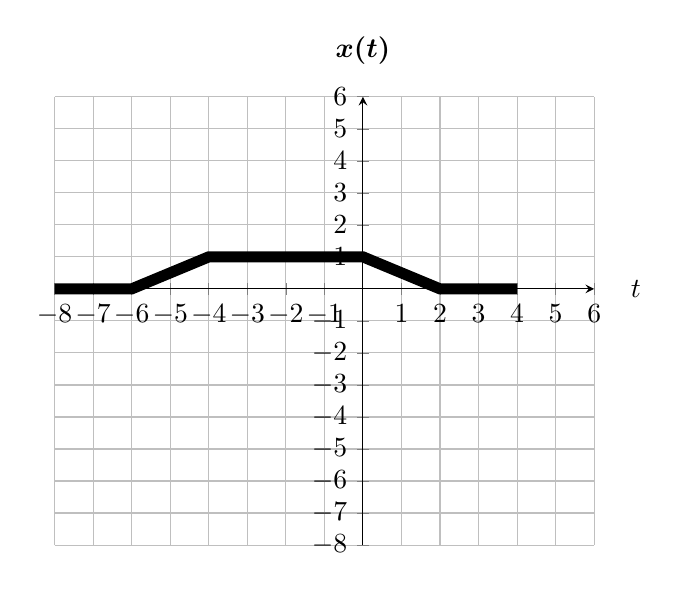
\begin{tikzpicture}[scale=1.0]
           \begin{axis}[
          axis lines=middle,
          xlabel={$t$},
          ylabel={$\boldsymbol{x(t)}$},
          xtick={-8,-7,-6,-5,-4, -3, ..., 6},
          ytick={-8,-7,-6 ,-5 ,-4, -3, ..., 6},
          ymin=-8, ymax=6,
          xmin=-8, xmax=6,
          every axis x label/.style={at={(ticklabel* cs:1.05)}, anchor=west,},
          every axis y label/.style={at={(ticklabel* cs:1.05)}, anchor=south,},
          grid,
        ]
            \path[draw,line width=4pt]  (-8,0) -- (-6,0) -- (-4,1) -- (-3,1) -- (-2,1) -- (-1,1) -- (0,1) -- (1,0.5) -- (2,0) -- (4,0);
           \end{axis}
        \end{tikzpicture}
        \caption{Graph of $y(t)=x(1/2t+1)$}
        \label{fig:q2}
    \end{figure}

\item      
    \begin{enumerate}
    \item 
    Figure 3 represents the solution for question 3.a . \\
        \begin{figure}[H]
            \centering
            \begin{tikzpicture}[scale=1.0]
               \begin{axis}[
              axis lines=middle,
              xlabel={$n$},
              ylabel={$\boldsymbol{x[n]}$},
              xtick={-8,-7,-6,-5,-4, -3, ..., 6},
              ytick={-8,-7,-6 ,-5 ,-4, -3, ..., 6},
              ymin=-8, ymax=6,
              xmin=-8, xmax=6,
              every axis x label/.style={at={(ticklabel* cs:1.05)}, anchor=west,},
              every axis y label/.style={at={(ticklabel* cs:1.05)}, anchor=south,},
              grid,
            ]
                \addplot [ycomb,black, thick, mark=*] table [x={n}, y={xn}] {q3a.dat};
               \end{axis}
            \end{tikzpicture}
            \caption{Graph of $ y[n] = x[-n] + x[2n+1]$}
            \label{fig:q3}
        \end{figure}
    \item 
    $x[-n] + x[2n+1] = 3\delta (n+7) - 4\delta(n+4) + 2\delta (n+2) - \delta(n+1) - \delta (n) + 3 \delta(n-3)$ \\
    \end{enumerate}

\item 
    $ x(t)=A*cos(wt-k)  \xrightarrow{} T_0 = 2\pi/w_0 $\\
    $ x(n)=A*cos(\Omega n-k) \xrightarrow{} N_0=m \times 2\pi/\Omega_0 $\\
    Shifting does not effect period
    \begin{enumerate}
    \item %write the solution of q4a
        period of cos $\rightarrow{}  m \times 2\pi/(13\pi/10) = m \times 20/13 \rightarrow{}_{m=13} N_0=20$ \\
        period of sin $ \rightarrow{}  m \times 2\pi/(7\pi/3) = m \times 6/7 \rightarrow{}_{m=7} N_0=6$ \\
        LCM(20,6)=60
    \item %write the solution of q4b
        $N=m\times2\pi/3$ there is no integer m that makes N integer, so this signal is not periodic.
    \item %write the solution of q4c
        $T=2\pi/3=2/3$
    \item %write the solution of q4d
    $x(t)=-je^{j5t}=-jcos(5t)+sin(5t)$\\
    period of sin and cos $\rightarrow{} T=2\pi/5$\\
    LCM($2\pi/5,2\pi/5$)=$2\pi/5$
    \end{enumerate}

\item %write the solution of q5
Since $x(n)\neq x(-n)$ and $x(n)\neq -x(-n)$ for all n the signal is not even and not odd.\\
$odd\{x(n)\}=0.5\{x(n)-x(-n)\}$\\
$even\{x(n)\}=0.5\{x(n)+x(-n)\}$\\
$x(n)=-\delta(n-1)+2\delta(n-2)-4\delta(n-4)+3\delta(n-7)$\\
$\delta(-n-k)=\delta(n+k)$\\
fill the equations and you get\\
$odd\{x(n)\}=0.5*(-\delta(n-1)+2\delta(n-2)-4\delta(n-4)+3\delta(n-7) +\delta(n+1)-2\delta(n+2)+4\delta(n+4)-3\delta(n+7))$\\
$even\{x(n)\}=0.5*(-\delta(n-1)+2\delta(n-2)-4\delta(n-4)+3\delta(n-7) -\delta(n+1)+2\delta(n+2)-4\delta(n+4)+3\delta(n+7))$
\\
\begin{figure} [h!]
    \centering
    \begin{tikzpicture}[scale=1.0] 
      \begin{axis}[
          axis lines=middle,
          xlabel={$n$},
          ylabel={$\boldsymbol{odd\{x[n]\}}$},
          xtick={ -8,-7, ..., 8},
          ytick={ -2,-1.5, -1,-0.5,0,0.5,1,1.5,2},
          ymin=-2, ymax=2,
          xmin=-8, xmax=8,
          every axis x label/.style={at={(ticklabel* cs:1.05)}, anchor=west,},
          every axis y label/.style={at={(ticklabel* cs:1.05)}, anchor=south,},
          grid,
        ]
        \addplot [ycomb, black, thick, mark=*] table [x={n}, y={xn}] {q5odd.dat};
      \end{axis}
    \end{tikzpicture}
    \caption{$n$ vs. $odd\{x(n)\}$.}
    \label{fig:q3}
\end{figure}
\begin{figure} [h!]
    \centering
    \begin{tikzpicture}[scale=1.0] 
      \begin{axis}[
          axis lines=middle,
          xlabel={$n$},
          ylabel={$\boldsymbol{even\{x[n]\}}$},
          xtick={ -8,-7, ..., 8},
          ytick={ -2,-1.5, -1,-0.5,0,0.5,1,1.5,2},
          ymin=-2, ymax=2,
          xmin=-8, xmax=8,
          every axis x label/.style={at={(ticklabel* cs:1.05)}, anchor=west,},
          every axis y label/.style={at={(ticklabel* cs:1.05)}, anchor=south,},
          grid,
        ]
        \addplot [ycomb, black, thick, mark=*] table [x={n}, y={xn}] {q5even.dat};
      \end{axis}
    \end{tikzpicture}
    \caption{$n$ vs. $even\{x(n)\}$.}
    \label{fig:q3}
\end{figure}

\newpage
\item 
    \begin{enumerate}
    \item %write the solution of q6a 
        \begin{itemize}
            \item has memory since for t $ \neq$ 3 present value of output is dependent on future or past values of input.
            \item stable since all bounded inputs generate bounded outputs.
            \item not causal since for t bigger than 3, output is represented by future values of input
            \item linear since the superposition principle holds $ \rightarrow{} $
                $y_1(t)=a_1x_1(2t-3)$ and $y_2(t)=a_2x_2(2t-3) \rightarrow{} y_3(t)=a_1x_1(2t-3)+a_2x_2(2t-3)=y_1(t)+y_2(t)$ 
            \item invertible since $y((t+3)/2)=x(2((t+3)/2)-3)=x(t)$
            \item time invariant since, shift input and output by $t_0 \rightarrow{} $ input becomes $x(2(t-t_0)-3)=x(2t-2t_0-3)$, output becomes $y(t-t_0)=x(2(t-t_0)-3)=x(2t-2t_0-3)$=input
        \end{itemize}
    \item %write the solution of q6b
        \begin{itemize}
            \item memoryless since present value of output is represented by only present values of input
            \item not stable since output is dependent on input and time, so we can't ensure boundedness of output for bounded inputs.
            \item causal since present value of output is represented by only present values of input.
            \item linear since the superposition principle holds $ \rightarrow{} $
                $y_1(t)=a_1tx_1(t)$ and $y_2(t)=a_2tx_2(t) \rightarrow{} y_3(t)=t(a_1x_1(t)+a_2x_2(t)=y_1(t)+y_2(t)$ 
            \item invertible since $y(t)/t=x(t)$
            \item time invariant since, shift input and output by $t_0 \rightarrow{} $ input becomes $x(t-t_0)$, output becomes $y(t-t_0)=(t-t_0)x(t-t_0)\neq$input
        \end{itemize}
    \item %write the solution of q6c
        \begin{itemize}
            \item has memory since for n $\neq$ 3, present value of output is represented by future or past values of input.
            \item stable since all bounded inputs generate bounded outputs.
            \item not causal since for n bigger than 3, output is represented by future values of input
            \item linear since the superposition principle holds $ \rightarrow{} $
                $y_1(n)=a_1x_1(2n-3)$ and $y_2(n)=a_2x_2(2n-3) \rightarrow{} y_3(n)=a_1x_1(2n-3)+a_2x_2(2n-3)=y_1(n)+y_2(n)$ 
            \item invertible since $y((n+3)/2)=x(2((n+3)/2)-3)=x(n)$
            \item time invariant since, shift input and output by $n_0 \rightarrow{} $ input becomes $x(2(n-n_0)-3)=x(2n-2n_0-3)$, output becomes $y(n-n_0)=x(2(n-n_0)-3)=x(2n-2n_0-3)$=input
        \end{itemize}
    \item %write the solution of q6d
        \begin{itemize}
            \item has memory since present value of output is represented by past values of input(sum of all past inputs).
            \item not stable since sum of all past input values can be unbounded, making output unbounded (even if all input values are bounded).
            \item causal since present value of output depends on only past values of input. 
            \item linear since the superposition principle holds $ \rightarrow{} $
                $y_1(n)=a_1 \sum_{k=1}^{\infty}{x_1(n-k)}$ and $y_2(n)=a_2 \sum_{k=1}^{\infty}{x_2(n-k)} \rightarrow{} y_3(n)= \sum_{k=1}^{\infty}{a_1x_1(n-k)+a_2x_2(n-k)}=y_1(n)+y_2(n)$ 
            \item invertible since $y(n+1)-y(n)=\{x(n)+x(n-1)+x(n-2)...\}-\{x(n-1)+x(n-2),...\}=x(n)$
            \item time invariant since, shift input and output by $n_0 \rightarrow{} $ input becomes $\sum_{k=1}^{\infty}{x(n-n_0-k)}$, output becomes $y(n-n_0)= \sum_{k=1}^{\infty}{x(n-n_0-k)}$=input
        \end{itemize}
    \end{enumerate}


\end{enumerate}
\end{document}

